\input{head.inc}
  
% Präambelbefehle für die Präsentation
\title[TET: Beliebig veränderliche Felder- Energieerhaltung]{Beliebig veränderliche Felder- Energieerhaltung}

\begin{document}
% 
% Frontmatter 
% 
%%%%%%%%%%%%%%%%%%%%%%%%%%%%%%%%%%%%%%%%%%%%%%%%%%%%%%%%%%%%%%%%%%%%%%%%%%%%%%%%%%%%%%%%%%%%%%%%%%%%%%%%%%%%%%%%%%%%%%%%%%%%% 

%% inserts the title page and the table of contents
\maketitle

% 
% Content 
% 
%%%%%%%%%%%%%%%%%%%%%%%%%%%%%%%%%%%%%%%%%%%%%%%%%%%%%%%%%%%%%%%%%%%%%%%%%%%%%%%%%%%%%%%%%%%%%%%%%%%%%%%%%%%%%%%%%%%%%%%%%%%%% 
\section{Beliebig veränderliche Felder- Energieerhaltung}

\begin{frame}
  \frametitle{Maxwellgleichungen -- Ladungserhaltung}
  \begin{itemize}[<+->]
  \item Wir betrachten nun den \alert{vollständigen Satz der Maxwell-Gleichungen}:
    \begin{align*}
      \divergenz \verschiebung[v] & = \laddichte{V} & \rotation \efeld[v] &= - \frac{\partial \tetB[v]}{\partial t}\\
      \divergenz \tetB[v] &= 0 & \rotation\magfeld[v] &= \elstromdichte[v] + \frac{\partial \verschiebung[v]}{\partial t}
    \end{align*}
  \item \alert{lineare, homogene und isotrope} Medien und \alert{lokales Ohmsches Gesetz}
    $$
    \verschiebung[v] = \varepsilon \efeld[v] \qquad \tetB[v] = \mu \magfeld[v] \qquad \elstromdichte[v] = \kappa\efeld[v]
    $$
  \item \alert{Ladungserhaltung} (eigentlich axiomatisch vorausgesetzt) folgt direkt aus den Maxwell-Gleichungen:
    \begin{align*}
      \divergenz (\rotation\magfeld[v]) = 0 &= \divergenz \elstromdichte[v] + \divergenz\dfrac{\partial \verschiebung[v]}{\partial t}
      = \divergenz \elstromdichte[v] + \dfrac{\partial \divergenz \verschiebung[v]}{\partial t} = \divergenz \elstromdichte[v] + \dfrac{\partial \laddichte{V}}{\partial t}\\
      \Aboxed{\divergenz \elstromdichte[v] + \dfrac{\partial\laddichte{V}}{\partial t} &= 0} \text{ Kontinuitätsgleichung (lokal)}\\
      \Aboxed{\oiint_{O(V)}\elstromdichte[v]\cdot\upd\vec{A} + \dfrac{\partial}{\partial t} \iiint_V \laddichte{V}\upd V &= 0} \text{ Kontinuitätsgleichung (integral)}      
    \end{align*}
  \end{itemize}
\end{frame}


\begin{frame}
  \frametitle{Energieerhaltung}
  \begin{itemize}[<+->]
  \item Betrachte bewegte Ladung $q = \laddichte{V}\upd V$, Geschwindigkeit $\vec{v}$ ($|\vec{v}| \ll c$)
  \item Lorenzkraft:
    $$
    \vec{F} = q \left( \efeld[v] + \vec{v} \times \tetB[v]\right) \to \upd\vec{F} = \laddichte{V}\upd V \left( \efeld[v] + \vec{v} \times \tetB[v]\right) 
    $$
  \item Differentielle \alert{verrichtete Arbeit} $\upd W$ bei Verschiebung um $\Delta\vec{s} = \vec{v} \Delta t$:
    $$
      \upd W =  \upd\vec{F} \cdot \Delta\vec{s} = \laddichte{V}\upd V \left( \efeld[v] + \vec{v} \times \tetB[v]\right)\cdot \Delta\vec{s}
      = \laddichte{V}\upd V\, \efeld[v] \cdot \Delta\vec{s} = \laddichte{V}\upd V\, \efeld[v] \cdot \vec{v} \Delta t
    $$
  \item Differentielle \alert{Leistung} $\upd\left( \frac{W}{\Delta t}\right)$:
    $$
    \upd\left( \frac{W}{\Delta t}\right) = \laddichte{V}\vec{v}\cdot\efeld[v]\, \upd V = \elstromdichte[v]\cdot\efeld[v]\, \upd V
    $$
  \item Hiermit ergibt sich die \alert{Leistung} zu
    $$
    P = \frac{W}{\Delta t} = \iiint_V \elstromdichte[v]\cdot\efeld[v]\, \upd V \text{ (analog zu } P=U\cdot I \text{ im Leiter)}
    $$
    \item \alert{Verlustleistungsdichte} $p_V=\elstromdichte[v]\cdot\efeld[v]$ $\to$ Stationäres elektrisches Strömungsfeld
  \end{itemize}
\end{frame}

\begin{frame}
  \frametitle{Energieerhaltung -- Poyntingscher Satz}
  \begin{itemize}[<+->]
  \item Weitere Betrachtung der Verlustleistungsdichte $p_V=\elstromdichte[v]\cdot\efeld[v]$:
    $$
    p_V = \elstromdichte[v]\cdot\efeld[v] = \efeld[v] \cdot \elstromdichte[v] = \efeld[v] \cdot \left(\rotation\magfeld[v] - \frac{\partial \verschiebung[v]}{\partial t}\right) =  \textcolor{red}{\efeld[v] \cdot \rotation\magfeld[v]} - \efeld[v] \cdot \frac{\partial \verschiebung[v]}{\partial t}  
    $$
  \item Es gilt weiterhin:
    $$
    \divergenz \left(\efeld[v] \times \magfeld[v]\right) = \magfeld[v]\cdot\rotation\efeld[v] - \textcolor{red}{\efeld[v] \cdot \rotation\magfeld[v]} = - \magfeld[v]\cdot\frac{\partial \tetB[v]}{\partial t} - \textcolor{red}{\efeld[v] \cdot \rotation\magfeld[v]}
    $$
  \item Somit ergibt sich der \alert{Poyntingsche Satz} in differentieller Form:
    $$
    \boxed{\efeld[v] \cdot \elstromdichte[v] = - \divergenz \left(\efeld[v] \times \magfeld[v]\right) - \magfeld[v]\cdot\frac{\partial \tetB[v]}{\partial t} - \efeld[v] \cdot \frac{\partial \verschiebung[v]}{\partial t} } \text{ allgemein}
    $$
    \item Für $\verschiebung[v] = \varepsilon \efeld[v]$ und $\tetB[v] = \mu \magfeld[v]$ folgt
    $$
    \boxed{\efeld[v] \cdot \elstromdichte[v] = - \divergenz \left(\efeld[v] \times \magfeld[v]\right) - \frac{\partial}{\partial t}\left[\frac{1}{2} \magfeld[v]\cdot\tetB[v] + \frac{1}{2} \efeld[v] \cdot \verschiebung[v]\right] } \text{ lineare, homogene, isotrope Medien}
    $$
  \end{itemize}
\end{frame}

\begin{frame}
  \frametitle{Energieerhaltung -- Poyntingscher Satz (fortgesetzt)}
  \begin{itemize}[<+->]
  \item Wir betrachten die Terme im Poytingschen Satz
    $$
    \boxed{\efeld[v] \cdot \elstromdichte[v] = - \divergenz \left(\efeld[v] \times \magfeld[v]\right) - \frac{\partial}{\partial t}\left[\frac{1}{2} \magfeld[v]\cdot\tetB[v] + \frac{1}{2} \efeld[v] \cdot \verschiebung[v]\right] } \text{ lineare, homogene, isotrope Medien}
    $$
  \item Joulsche Wärme $\efeld[v] \cdot \elstromdichte[v]$ $\to$ Stationäres el. Strömungsfeld
  \item Elektrische Energiedichte $\frac{1}{2} \efeld[v] \cdot \verschiebung[v]$ $\to$ Elektrostatik VIII - Materie
  \item Magnetische Energiedichte $\frac{1}{2} \magfeld[v]\cdot\tetB[v]$ $\to$ Magnetostatik I - Grundlagen
  \item Offenbar ist die gesamte \alert{elektromagnetische Energiedichte} (lineare, isotrope, homogene Medien)
    $$
    \boxed{w_{em} = w_e + w_m = \frac{1}{2} \magfeld[v]\cdot\tetB[v] + \frac{1}{2} \efeld[v] \cdot \verschiebung[v]}
    $$ 
  \end{itemize}
\end{frame}

\begin{frame}
  \frametitle{Energieerhaltung -- Poyntingscher Satz (fortgesetzt)}
  \begin{itemize}[<+->]
  \item Differentielle Dartstellung
    $$
    \efeld[v] \cdot \elstromdichte[v] = - \divergenz \left(\efeld[v] \times \magfeld[v]\right) - \frac{\partial}{\partial t}\left[\frac{1}{2} \magfeld[v]\cdot\tetB[v] + \frac{1}{2} \efeld[v] \cdot \verschiebung[v]\right] = - \divergenz \left(\efeld[v] \times \magfeld[v]\right) - \frac{\partial w_{em}}{\partial t} 
    $$
  \item Übergang zur integralen Darstellung $\to$ Volumenintegral:
    \begin{align*}
      \underbrace{\frac{W}{\Delta t} = \iiint_V \efeld[v] \cdot \elstromdichte[v] \upd V}_{\text{mechanisch, thermodynamisch}} &= \underbrace{- \oiint_{O(V)} \efeld[v] \times \magfeld[v] \cdot \upd\vec{A} - \frac{\partial}{\partial t} \iiint_V w_{em} \upd V}_{elektrisch}\\
      \frac{\partial}{\partial t} \iiint_V w_{mech} \upd V &= - \oiint_{O(V)} \efeld[v] \times \magfeld[v] \cdot \upd\vec{A} - \frac{\partial}{\partial t} \iiint_V w_{em} \upd V\\
      \Aboxed{\frac{\partial}{\partial t} \iiint_V \left( w_{mech} + w_{em} \right) \upd V &= - \oiint_{O(V)} \efeld[v] \times \magfeld[v] \cdot \upd\vec{A}} \text{ \alert{integraler Poyntigscher Satz}} 
      \end{align*}
  \end{itemize}
\end{frame}

\begin{frame}
  \frametitle{Energieerhaltung -- Poynting-Vektor}
  \begin{itemize}[<+->]
  \item Integraler Poyntingscher Satz
    $$
    \frac{\partial}{\partial t} \iiint_V \left( w_{mech} + w_{em} \right) \upd V = - \oiint_{O(V)} \efeld[v] \times \magfeld[v] \cdot \upd\vec{A}
    $$
  \item Änderung der Energie im Volumen $V$ entspricht dem Fluss des Vektors $\poyvec[v]= \efeld[v] \times \magfeld[v]$ durch die Oberfläche des Volumens $O(V)$.
  \item Die Größe
    $$
    \boxed{\poyvec[v]= \efeld[v] \times \magfeld[v]} \quad [\poyvec[v]] = \si{\watt\per\metre\squared}
    $$
    ist die lokale \alert{Energieflussdichte} oder der \alert{Poynting-Vektor}.
  \item Hiermit schreiben sich integraler und differentieller Poyntingscher Satz wie folgt:
    \begin{align*}
      \Aboxed{\frac{\partial}{\partial t} \iiint_V \left( w_{mech} + w_{em} \right) \upd V + \oiint_{O(V)} \poyvec[v] \cdot \upd\vec{A} &= 0}\\
      \Aboxed{\frac{\partial}{\partial t} \left( w_{mech} + w_{em} \right) + \divergenz\poyvec[v] &=0}
      \end{align*}
  \end{itemize}
\end{frame}

\begin{frame}
  \frametitle{Energieerhaltung -- harmonische Zeitabhängigkeit}
  \begin{itemize}[<+->]
  \item Harmonische Zeitabhängigkeit: ($\to$ Quasistationäre Felder - Grundlagen)
    $$
    	\efeld[v](\ortsvektor[v],\,t) = \real{\efeld[uv](\ortsvektor[v])  \euler^{\komplex  \omega  t} } = \frac{1}{2} \left[\efeld[uv](\ortsvektor[v])  \euler^{\komplex  \omega  t}  + \efeld[uv]^\star(\ortsvektor[v])  \euler^{-\komplex  \omega  t}  \right] 
        $$
      \item Anwendung für $w_e = \frac{1}{2} \efeld[v] \cdot \verschiebung[v]$:
        \begin{align*}
          w_e &= \frac{1}{2} \efeld[v] \cdot \verschiebung[v] \\
              &= \frac{1}{2} \left[ \frac{1}{2} \left(\efeld[uv]  \euler^{\komplex  \omega  t}  + \efeld[uv]^\star  \euler^{-\komplex  \omega  t}  \right)\right] \cdot \left[ \frac{1}{2} \left(\verschiebung[uv]  \euler^{\komplex  \omega  t}  + \verschiebung[uv]^\star  \euler^{-\komplex  \omega  t}  \right)  \right] \\
              &= \frac{1}{8} \left[ \efeld[uv] \cdot \verschiebung[uv]  \euler^{\komplex  2\omega  t} + \efeld[uv]^\star \cdot \verschiebung[uv]^\star  \euler^{-\komplex  2\omega  t}\right] +  \frac{1}{8} \left[ \efeld[uv] \cdot \verschiebung[uv]^\star  + \efeld[uv]^\star \cdot \verschiebung[uv] \right]\\
          &=\frac{1}{4}\real{\efeld[uv] \cdot \verschiebung[uv]  \euler^{\komplex  2\omega  t}} + \frac{1}{4}\real{\efeld[uv] \cdot \verschiebung[uv]^\star}
        \end{align*}
      \item Mittelwert über eine Periode:
        $$
        \boxed{\langle w_e \rangle = \frac{1}{4}\real{\efeld[uv] \cdot \verschiebung[uv]^\star} = \underbrace{\frac{1}{4}\efeld[uv] \cdot \verschiebung[uv]^\star}_{(\verschiebung[v]=\varepsilon\efeld[v]), \varepsilon\in \mathbb{R}}} \pause\text{ analog } \boxed{\langle w_m \rangle = \frac{1}{4}\real{\magfeld[uv] \cdot \tetB[uv]^\star} = \underbrace{\frac{1}{4}\magfeld[uv] \cdot \tetB[uv]^\star}_{(\tetB[v]=\mu\magfeld[v]), \mu\in \mathbb{R}}}
        $$
  \end{itemize}
\end{frame}

\begin{frame}
  \frametitle{Mittelwerte -- komplexer Poynting-Vektor}
  \begin{itemize}[<+->]
  \item zeitliche Mittelwerte:
    \begin{align*}
      \langle w_e \rangle & = \frac{1}{4}\real{\efeld[uv] \cdot \verschiebung[uv]^\star} = \underbrace{\frac{1}{4}\efeld[uv] \cdot \verschiebung[uv]^\star}_{(\verschiebung[v]=\varepsilon\efeld[v]), \varepsilon\in \mathbb{R}}\\
      \langle w_m \rangle & = \frac{1}{4}\real{\magfeld[uv] \cdot \tetB[uv]^\star} = \underbrace{\frac{1}{4}\magfeld[uv] \cdot \tetB[uv]^\star}_{(\tetB[v]=\mu\magfeld[v]), \mu\in \mathbb{R}} \\
      \langle p_V \rangle & = \frac{1}{2}\real{\efeld[uv] \cdot \elstromdichte[uv]^\star} = \underbrace{\frac{1}{2}\efeld[uv] \cdot \elstromdichte[uv]^\star}_{(\elstromdichte[v]=\kappa\efeld[v]), \kappa\in \mathbb{R}}\\
      \Aboxed{\langle \poyvec[v]\rangle &= \frac{1}{2}\real{\efeld[uv] \times \magfeld[uv]^\star}} = \real{\poyvec[uv]}
    \end{align*}
  \item Hierbei wird der \alert{komplexe Poyntingsche Vektor} $\poyvec[uv]$ eingeführt:
    $$
    \boxed{\poyvec[uv] = \frac{1}{2}\efeld[uv] \times \magfeld[uv]^\star} \text{ komplexer Poynting-Vektor} 
    $$
  \end{itemize}
\end{frame}

\begin{frame}
  \frametitle{komplexer Poyntingscher-Satz (differentiell)}
  \begin{itemize}[<+->]
  \item Wir bilden die Divergenz des komplexen Poynting-Vektor $\poyvec[uv] = \frac{1}{2}\efeld[uv] \times \magfeld[uv]^\star$:
    \begin{align*}
      \divergenz (\frac{1}{2}\efeld[uv] \times \magfeld[uv]^\star) &= \frac{1}{2} \left( \magfeld[uv]^\star\cdot\rotation \efeld[uv] - \efeld[uv]\cdot\rotation \magfeld[uv]^\star\right)\\
                                                                   &= \frac{1}{2} \left( \magfeld[uv]^\star\cdot (-\komplex\omega\tetB[uv]) - \efeld[uv]\cdot (\elstromdichte[uv]+\komplex\omega\verschiebung[uv])^\star \right) \\
                                                                   &= \frac{1}{2} \left( -\komplex\omega\magfeld[uv]^\star\cdot \tetB[uv] - \efeld[uv]\cdot \elstromdichte[uv]^\star + \komplex\omega\efeld[uv]\cdot \verschiebung[uv]^\star \right)
    \end{align*}
  \item Insgesamt gilt somit der \alert{komplexe Poyntingsche Satz} in differentieller Form
    \begin{align*}
      \divergenz\poyvec[uv] &&+&& \frac{1}{2} \efeld[uv]\cdot \elstromdichte[uv]^\star &&+&& \komplex 2\omega&&\Big[&&\frac{1}{4} \magfeld[uv]^\star\cdot\tetB[uv] &&-&& \frac{1}{4} \efeld[uv]\cdot \verschiebung[uv]^\star &&\Big] &&=&&0 \\
      \Leftrightarrow\divergenz\poyvec[uv] &&+&& \langle p_V \rangle &&+&& \komplex 2\omega&&\Big[&& \langle w_m\rangle &&-&& \langle w_e\rangle &&\Big] &&=&& 0
    \end{align*}
  \item Aufspaltung in Real- und Imaginärteil (Mittelwerte sind reele Werte):
    $$
    \real{\divergenz\poyvec[uv]} + \underbrace{\frac{1}{2} \efeld[uv]\cdot \elstromdichte[uv]^\star}_{\langle p_V \rangle} =0 \quad  \imaginaer{\divergenz\poyvec[uv]} + 2\omega\Bigg[\underbrace{\frac{1}{4} \magfeld[uv]\cdot\tetB[uv]^\star}_{\langle w_m\rangle} - \underbrace{\frac{1}{4} \efeld[uv]\cdot \verschiebung[uv]^\star}_{\langle w_e\rangle} \Bigg] =0 
    $$
  \end{itemize}
\end{frame}

\begin{frame}
  \frametitle{komplexer Poyntingscher-Satz (integral)}
  \begin{itemize}[<+->]
  \item Aus der differentielle Form folgt sofort der \alert{integrale komplexe Poyntingsche Satz}:
    \begin{align*}
      \divergenz\poyvec[uv] + \langle p_V \rangle + \komplex 2\omega\Big[ \langle w_m\rangle - \langle w_e\rangle \Big] &= 0\\
      \Leftrightarrow \Aboxed{\oiint_{O(V)} \poyvec[uv]\cdot \upd\vec{A} + \iiint_V \langle p_V \rangle \upd V + \komplex 2\omega\iiint_V \left( \langle w_m\rangle - \langle w_e\rangle \right)\upd V  &= 0}
    \end{align*}
  \item Der Realteil entspricht der mittleren \alert{Wirkleistung} (umgesetzte Energie, Ohmschen Verluste):
    $$
    \langle P_V \rangle = \iiint_V \langle p_V \rangle \upd V = -\oiint_{O(V)} \real{\poyvec[uv]}\cdot \upd\vec{A}
    $$
  \item Der Imaginärteil entspricht der mittleren \alert{Blindleistung}:
    $$
    2\omega\iiint_V \left( \langle w_m\rangle - \langle w_e\rangle \right)\upd V = -\oiint_{O(V)} \imaginaer{\poyvec[uv]}\cdot \upd\vec{A}
    $$
  \end{itemize}
\end{frame}

\begin{frame}
  \frametitle{Beispiel: Koaxialkabel}
  \begin{columns}
    \begin{column}{.5\linewidth}
      \resizebox{.7\columnwidth}{!}{\vbox{%
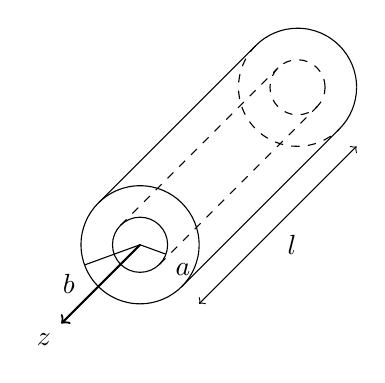
\begin{tikzpicture}
	% Achsen zeichnen
	\draw[->,thick] (0,0) -- (-1,-1) node [below left] {$z$};
	%Plot
	\draw (0,0) circle (.35);
	\draw (0,0) circle (.75);
	\draw (0,0) -- (340:.35) node [below right] {$a$};
	\draw (0,0) -- (200:.75) node[below left] {$b$};
	\draw (135:.75) --+ (2,2);
	\draw[style=dashed] (135:.35) --+ (2,2);
	\draw[style=dashed] (315:.35) --+ (2,2);
	\draw (315:.75) --+ (2,2);
	\draw[style=dashed] (2,2) circle (.35);
	\draw (2,2) +(0:.75) arc (0:135:0.75) ;
	\draw[style=dashed] (2,2)+(135:.75) arc (135:315:.75);
	\draw (2,2) +(315:.75) arc (315:360:.75);
	\draw[<-] (.75,-0.75)--(1.75,0.25) node[below right] {$l$};
	\draw[->] (1.75,0.25)--(2.75,1.25);
      \end{tikzpicture}
      
\begin{tikzpicture}
	% Achsen zeichnen
	%\draw[->,thick] (0,0) -- (-1,-1) node [below left] {$z$};
	\draw[<->] (0,0)--(0,2) node[left] {$2b$} --(0,4);
	\draw[<->] (1,1.5)--(1,2) node[left] {$2a$} --(1,2.5);
	\draw (1.5,4)--(5.5,4);
	\draw (1.5,0)--(5.5,0)--(5.5,2);
	\draw[->] (1.5,2)--(7,2) node[right] {$z$};
	\draw (1.5,0)--(1.5,2);
	\draw (1.5,1) circle(.25);
	\draw[<-] (1.1,.75)--(1.1,1.25) node[below left] {$\spannung_0$};	
	\draw (1.9,1.5) rectangle (5,2.5);
	\draw[style=dashed] (1.9,2.5)--(1.9,4.2) node[above] {$0$};
	\draw[style=dashed] (3.5,2.5)--(3.5,4.2) node[above] {$z$};
	\draw[fill=black] (1.7,0) circle(.05);
	\draw[fill=black] (1.7,2) circle(.05);
	\draw[fill=black] (5.3,0) circle(.05);
	\draw[fill=black] (5.3,2) circle(.05);
	\draw[fill=white] (5.35,0.5) rectangle (5.65,1.5);
	\node[right] at (5.75,1) {$\elwiderstand$};
	\node[right] at (3,1.65) {$\kappa$};
	\node[right] at (3,-.3) {$\kappa_a \rightarrow \infty$};
	\node[right] at (3.2,.75) {$\spannung ( z)$};
	\draw[->] (3.2,1.3)--(3.2,0.2);
      \end{tikzpicture}
}}
      \end{column}
    \begin{column}{.5\linewidth}
\begin{itemize}[<+->]
\item Koaxialleitung mit ohmschen Verlusten nur im Innenleiter: $\kappa_a\to\infty$
\item Betrachtung bei tiefen Frequenzen: $l\ll\lambda$, $a\ll\delta$, $\omega L \ll R_i$
\item Strom ist konstant: $I=I(\rho,\varphi,z) = I_0$
\item Widerstand des Innenleiters bis Position $z$: $R_i(z)=\frac{z}{\kappa\cdot \pi a^2}$
\item Maschengleichungen:
  \begin{align*}
    \text{große Masche:} && U_0 &= R_i(l)I_0 + RI_0 \\
    \text{kleine Masche:} && U_0 &= U(z) + R_i(z)I_0 \\
    \to &&U(z) &= U_0\left(1-\frac{z}{l+\kappa\pi a^2 R} \right)
    \end{align*}
  \end{itemize}
    \end{column}
\end{columns}
\end{frame}

\begin{frame}
  \frametitle{Beispiel: Koaxialkabel (fortgesetzt)}
\begin{itemize}[<+->]
\item Magnetfeld im Innenleiter und im Zwischenraum (außen Null):
  $$
  \magfeld[v]^i = \magfeld_\varphi^i \vu{\varphi} = \frac{I_0}{2\pi a}\frac{\rho}{a} \vu{\varphi} \text{ und } \magfeld[v]^a = \magfeld_\varphi^a \vu{\varphi} = \frac{I_0}{2\pi \rho} \vu{\varphi}
  $$
\item Elektrisches Feld im Innenleiter nur $z$-Komponente: $\efeld[v]^i=\efeld_z^i \vu{z} = \frac{\elstromdichte_z}{\kappa}\vu{z}=\frac{I_0}{\kappa\pi a^2}\vu{z}$
\item Elektrisches Feld im Zwischenraum: Lösung der Laplace-Gleichung $\laplace \phi =0$:
  \begin{itemize}[<+->]
  \item In Zylinderkoordinaten:
    $$
    \frac{1}{\rho}\frac{\partial}{\partial \rho}\left(\rho\frac{\partial \phi}{\partial \rho}\right) + \frac{1}{\rho^2}\frac{\partial^2 \phi}{\partial \varphi^2} + \frac{\partial^2 \phi}{\partial z^2} =0 \to \text{ Separationsansatz} \to \efeld[v] = -\gradient\phi
    $$
  \item + Randbedingungen: $\efeld_z^a(\rho=a) = \efeld_z^i \text{ und } \efeld_z^a(\rho=b) = 0$
    \item + Anfangsbedingung: $U_0=\int_a^b \efeld_\rho(\rho, z=0)\upd\rho$
    \end{itemize}
  \item Das ergibt:
    $$
    \efeld_\rho^a = \frac{U_0}{\rho \ln\nicefrac{b}{a}}\left(1-\frac{z}{l+\kappa\pi a^2 R}\right) \quad \efeld_z^a = \frac{U_0 \ln\nicefrac{b}{\rho}}{\ln\nicefrac{b}{a}}\frac{1}{l+\kappa\pi a^2 R} 
    $$
  \end{itemize}
\end{frame}

\begin{frame}
  \frametitle{Beispiel: Koaxialkabel (fortgesetzt)}
\begin{itemize}[<+->]
\item Berechnung des komplexen Poynting Vektors aus den Feldern:
  \begin{align*}
    \poyvec[uv]^i &= \frac{1}{2} \efeld[uv]^i \times \magfeld[uv]^{i\star} = -\frac{1}{2} \efeld_z^i \magfeld_\varphi^i \vu{\rho}\\
    \poyvec[uv]^a &=\frac{1}{2} \efeld[uv]^a \times \magfeld[uv]^{a\star} = -\frac{1}{2} \efeld_z^a \magfeld_\varphi^a \vu{\rho} + \frac{1}{2} \efeld_\rho^a \magfeld_\varphi^{a\star} \vu{z}
  \end{align*}
\item $\poyvec[uv]^i$ und $\poyvec[uv]^a$ sind reel $\to$ nur Wirkleistung! ($\omega L$ wurde explizit vernachlässigt!)
\item radial nach innen fließende Energie:
  $$
  - 2\pi a \int_0^l \poyvec[uv]^i (\rho=a)\cdot\vu{\rho} \upd z = \frac{1}{2} R_i(l) I_0^2 \to \text{ Verlustleistung im Innenleiter}
  $$
\item im Zwischenraum axialer Energietransport:
  $$
  \int_a^b \poyvec[uv]^a (\rho) \cdot\vu{z} 2 \pi\rho\upd\rho = \frac{1}{2} I_0 U(z) 
  $$
\item Von der Quelle abgegebene Leistung ($z=0$):
  $$
  P = \frac{1}{2} I_0U(0) = \frac{1}{2} \frac{U_0^2}{R+R_i(l)}
  $$
  \end{itemize}
\end{frame}



\input{finalframe.inc}
   
\end{document}